\documentclass[12pt,letterpaper]{article}
\usepackage{fullpage}
\usepackage[top=2cm, bottom=4.5cm, left=2.5cm, right=2.5cm]{geometry}
\usepackage{amsmath,amsthm,amsfonts,amssymb,amscd}
\usepackage{lastpage}
\usepackage{enumerate}
\usepackage{fancyhdr}
\usepackage{mathrsfs}
\usepackage{xcolor}
\usepackage{graphicx}
\usepackage{listings}
\usepackage{hyperref}

\hypersetup{%
  colorlinks=true,
  linkcolor=blue,
  linkbordercolor={0 0 1}
}
 
\renewcommand\lstlistingname{Algorithm}
\renewcommand\lstlistlistingname{Algorithms}
\def\lstlistingautorefname{Alg.}

\lstdefinestyle{Python}{
    language        = Python,
    frame           = lines, 
    basicstyle      = \footnotesize,
    keywordstyle    = \color{blue},
    stringstyle     = \color{green},
    commentstyle    = \color{red}\ttfamily
}

\setlength{\parindent}{0.0in}
\setlength{\parskip}{0.05in}

% Edit these as appropriate
\newcommand\course{Computaitonal Physics}
\newcommand\hwnumber{4}                  % <-- homework number
\newcommand\NetIDa{Jiachen Wan N19996964}           % <-- NetID of person #1


\pagestyle{fancyplain}
\headheight 35pt
\lhead{\NetIDa}
\lhead{\NetIDa\\\NetIDb}                 % <-- Comment this line out for problem sets (make sure you are person #1)
\chead{\textbf{\Large Homework \hwnumber}}
\rhead{\course \\ \today}
\lfoot{}
\cfoot{}
\rfoot{\small\thepage}
\headsep 1.5em

\begin{document}

\section*{Problem 1}

\begin{enumerate}
  \item
   I wrote a code for adaptive Bulirsch–Stoer method, based on the code written by Newman. To make it adaptive, I used recursion. When $n>0$, I call the function again, with half the step size. When the accuracy is small enough, the function  will return the r at t+H. I then take H, the big step size, be 20, and let the system integrate. The result is below:
   
   \begin{figure}[h]
    \centering
    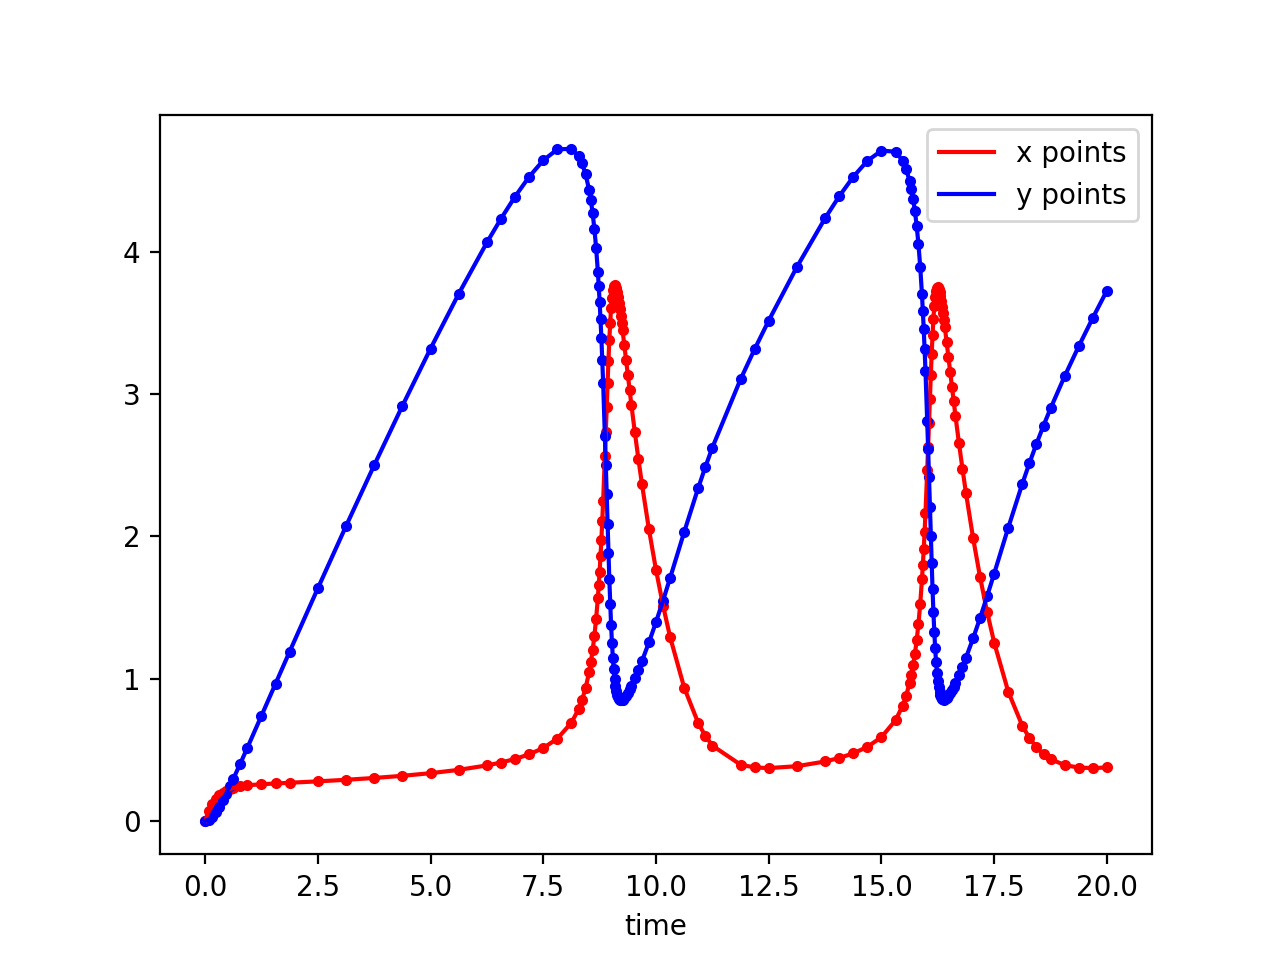
\includegraphics[width=1.\linewidth]{fig1a.png}
    \caption{Belousov–Zhabotinsky reaction simulation using adaptive Bulirsch–Stoer}
    \end{figure}
    We can clearly see that there are more points near local maxima or local minima, and less points when the behaviour is linear. This means that the adaptive method is taking effect, trying to spend more computing power at the region which the function's behaviour is complex.
    \clearpage
\end{enumerate}


\section*{Problem 2}
\begin{enumerate}
    \item
    Since we are not considering friction, the equation to solve is:
    \begin{equation}
        \frac{d^2r}{dt^2}=-\frac{GM}{4|r|^3}r
    \end{equation}
    Reduce it into a system of ODE in x and y components gives:
    \begin{equation}
        \frac{dv_x}{dt}=-\frac{GM}{4|r|^3}x
    \end{equation}
    \begin{equation}
        \frac{dv_y}{dt}=-\frac{GM}{4|r|^3}y
    \end{equation}
    \begin{equation}
        \frac{dx}{dt}=v_x
    \end{equation}
    \begin{equation}
        \frac{dy}{dt}=v_y
    \end{equation}    
    It has the form of gravitational pull, but with a factor of 1/4. Next, we are to simulate a elliptical orbit, such that the pericenter radius is  $10^{-7}$. The equation for velocity at apogee for a normal graviational pull is:
    \begin{equation}
        v_a=\sqrt{GM\frac{1-e}{a+c}}
    \end{equation}
    Relavent constants are defined by:
    \begin{figure}[h]
    \centering
    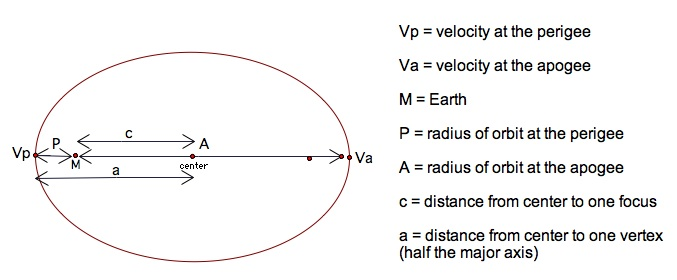
\includegraphics[width=1.\linewidth]{labeledellipse.jpg}
    \caption{Diagram for elliptical formula}
    \end{figure}
    \clearpage
    
    It is easy to see that:
    \begin{equation}
        v_a=\sqrt{2GM10^{-7}}
    \end{equation}
    But since our equation has an extra factor of 1/4, the actual velocity is:
    \begin{equation}
        v_a=\frac{1}{2}\sqrt{2GM10^{-7}}
    \end{equation}
    
    Using initial conditions x=1,y=0,$v_x=0$, and $v_y=v_a$, with $\delta=10^{-8}$ the following plot is obtained:
    \begin{figure}[h]
    \centering
    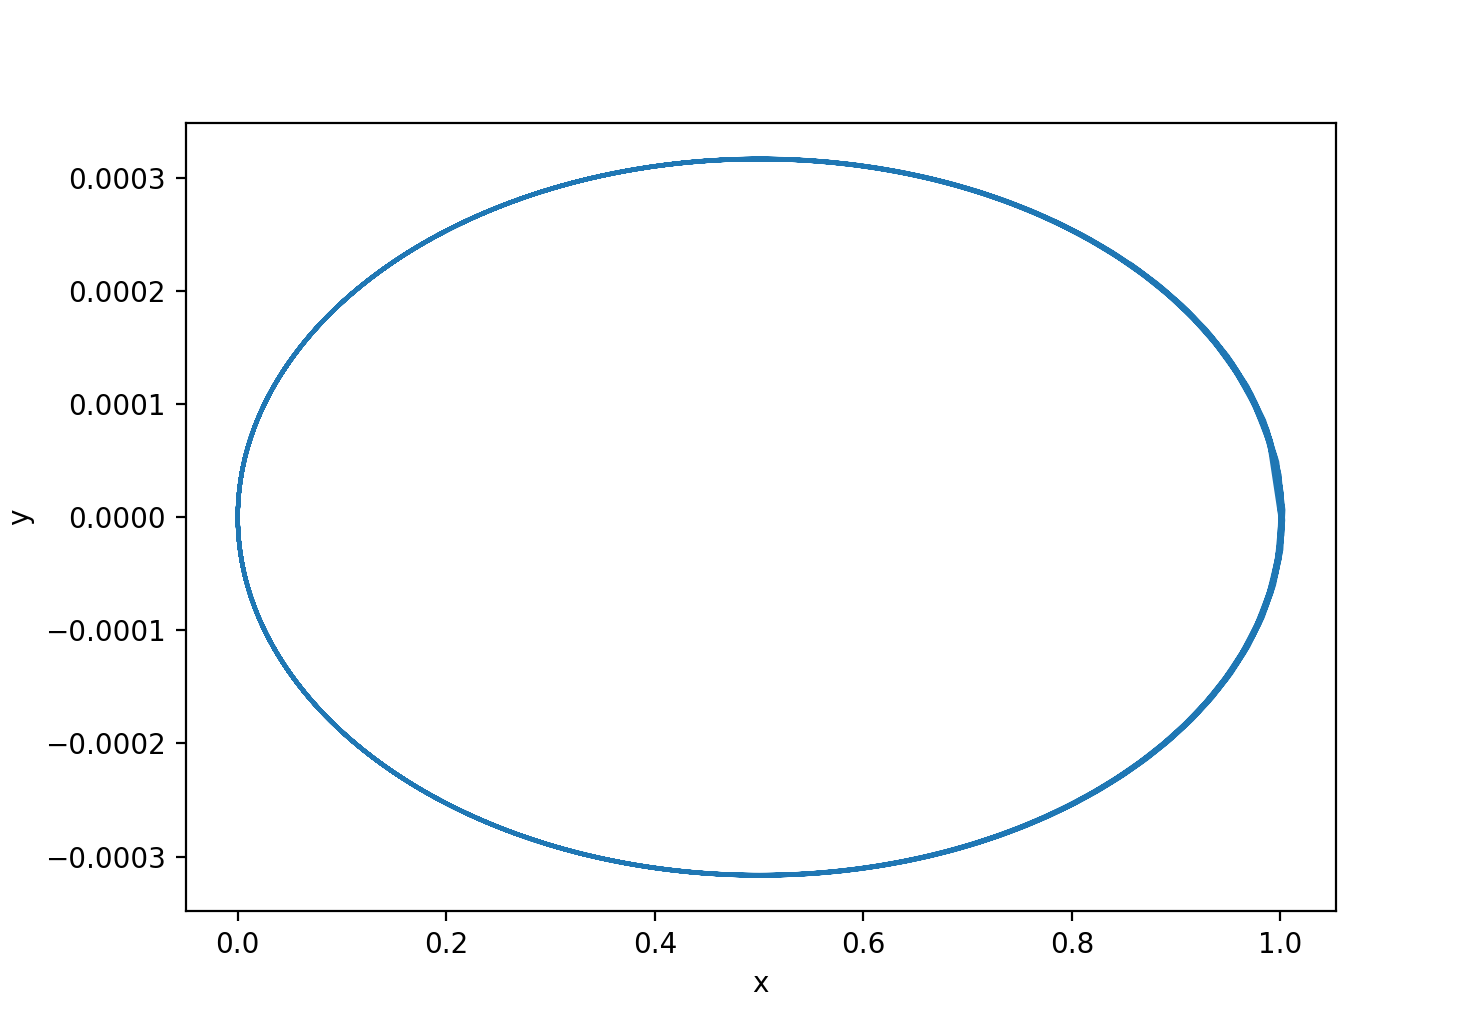
\includegraphics[width=1.\linewidth]{fig2a.png}
    \caption{The elliptical orbit resulted from the equation}
    \end{figure}
    The diagram looks different from the figure shown in class; one of the axis is different. However, assuming my code is correct (at least my adaptive RK4 code is correct, because I have tested the code with known result). So I couldn't figure out where went wrong. The result looks reasonable though.
    \clearpage
    So to further make sure my simulation is correct, I checked the smallest radius there is in the simulated trace:

    \begin{figure}[h]
    \centering
    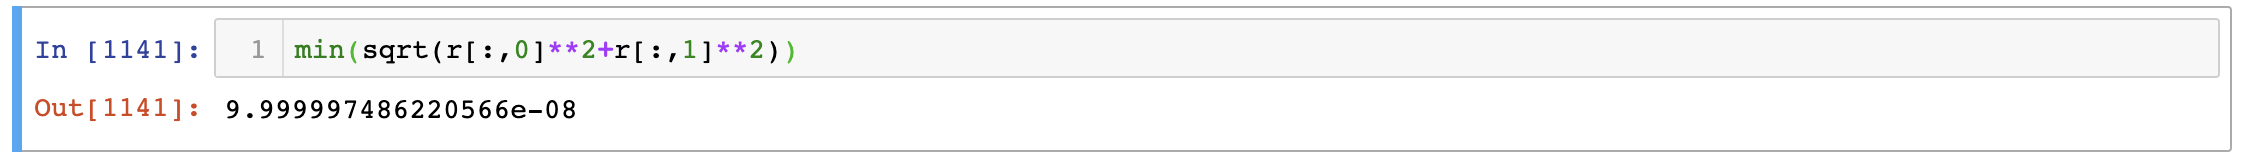
\includegraphics[width=1.\linewidth]{fig2b.png}
    \caption{Smallest radius from the simulated points}
    \end{figure}
    
    From this, it is clear that the pericenter radius is $10^{-7}$. With $\delta = 10^{-8}$, there is very little loss in accuracy. It can be shown by:
    
    \begin{figure}[h]
    \centering
    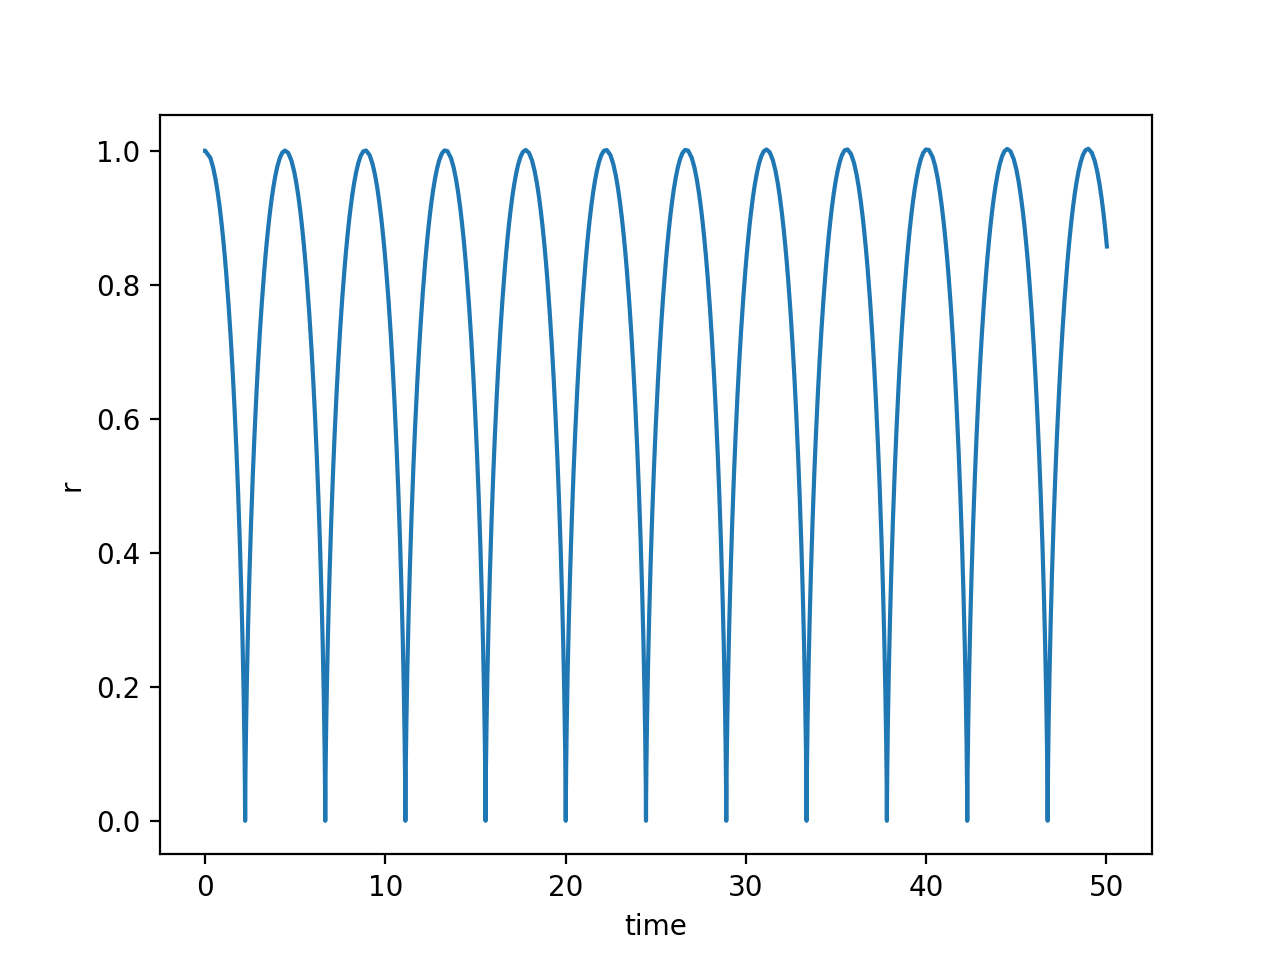
\includegraphics[width=1.\linewidth]{fig2c.png}
    \caption{Radius vs time}
    \end{figure}
    
    It can be clearly seen that there is barely any loss in accuracy. However, the period appears to be different from that was shown in class, and I have no idea why.
    \clearpage
    \item
    Now add in friction. A=B=1. The initial condition has changed as well, the initial velocity is 0.8 that of the velocity for circular orbit. The circular orbit velocity for our equation is:
    \begin{equation}
        v_{circle}=\frac{1}{2}\sqrt{\frac{GM}{r}}
    \end{equation}
    Using 0.8 times this as initial y velocity, the trace looks like:
    
    \begin{figure}[h]
    \centering
    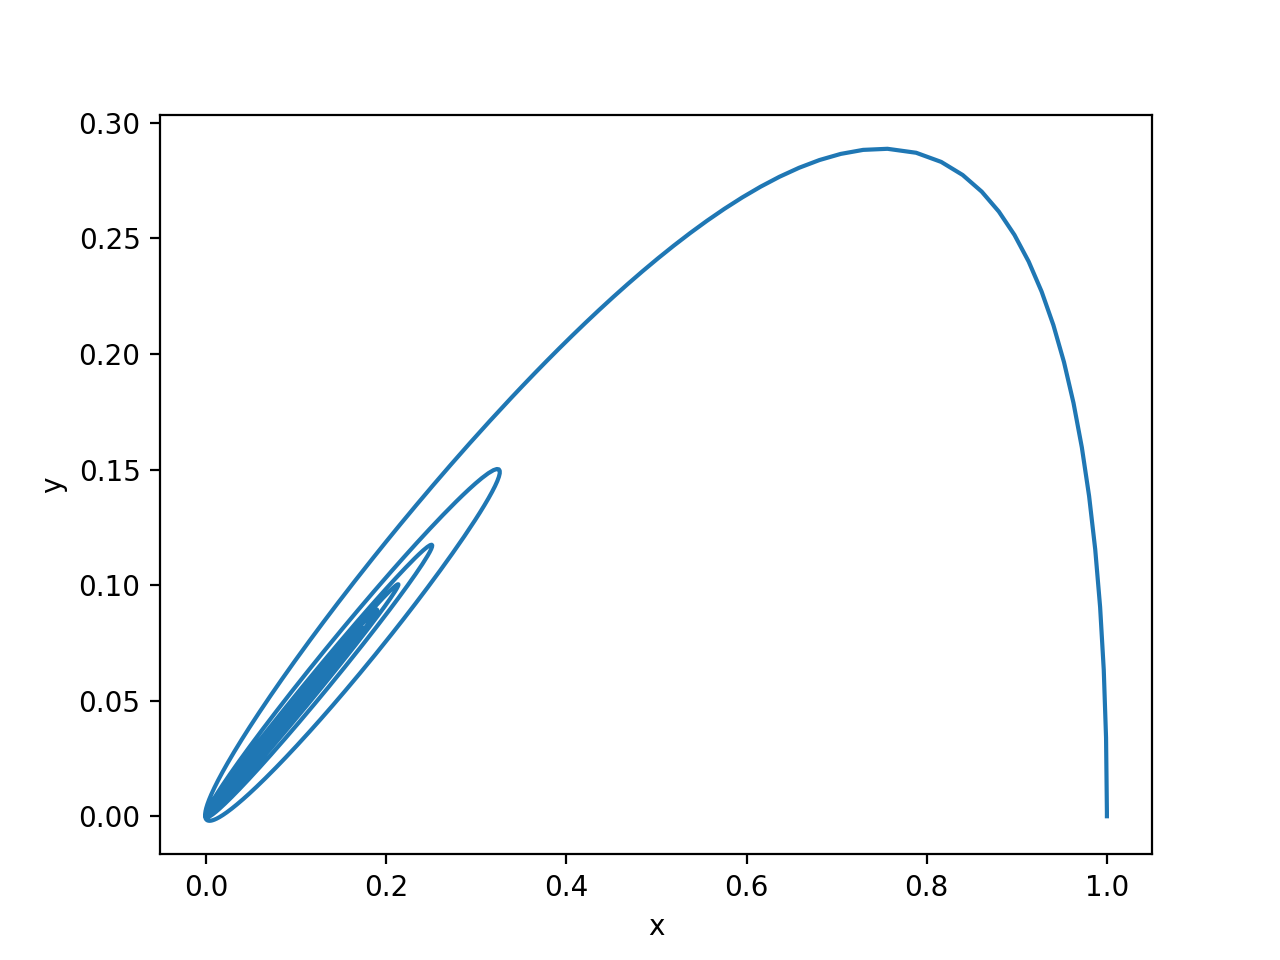
\includegraphics[width=1.\linewidth]{fig2d}
    \caption{A=B=1, trajectory}
    \end{figure}
    
    \clearpage
    Now, lets look at the log plot of radius against time:
    
    \begin{figure}[h]
    \centering
    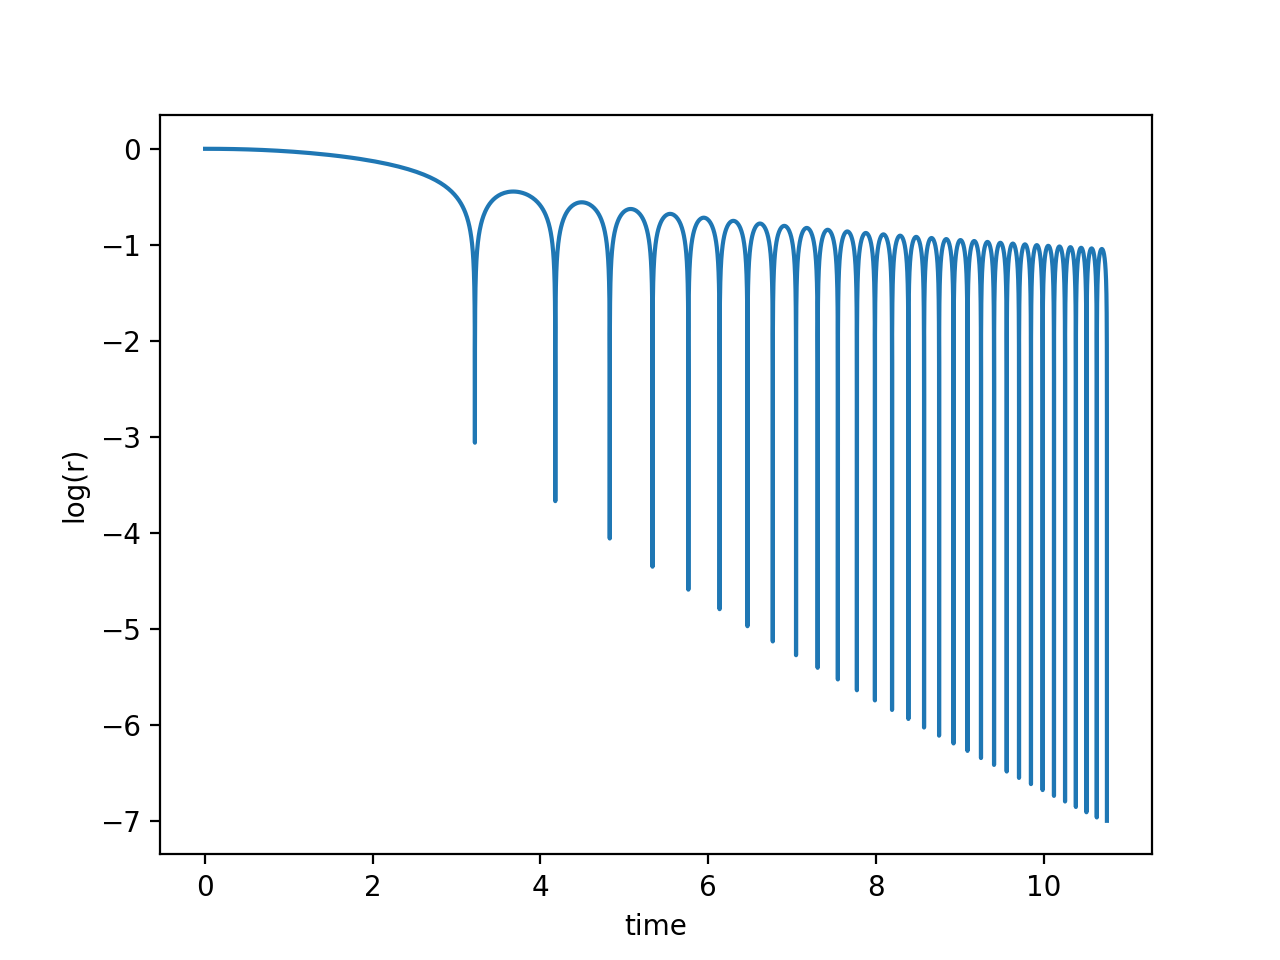
\includegraphics[width=1.\linewidth]{fig2e}
    \caption{A=B=1, log(r) against time}
    \end{figure}
    
    This figure has the expected behaviour. It is clearly seen that the black hole rotates towards the center, and eventually reaches the threshold of $10^{-7}$.
    
    \item
    From this equation,
    \begin{equation}
        \frac{d^2r}{dt^2}=-\frac{GM}{4|r|^3}r
    \end{equation}
    It is clear that $\frac{GM}{4|r|^3}$ has unit of $\frac{1}{s^2}$. 
    \begin{equation}
        \frac{GM}{4|r|^3}=\frac{6.67408*10^{-11} m^3 kg^{-1} s^{-2} 10^{8}*2*10^{30}kg }{(100*3.086*10^{16})^3}=3.6335*10^{-27}\frac{1}{s^2}
    \end{equation}
    So the unit for time is 0.5334 Myr, after manipulation.
    \clearpage
    The plot of time it takes for the black hole to reach $10^-7$ radius against B/A is below:
    \begin{figure}[h]
    \centering
    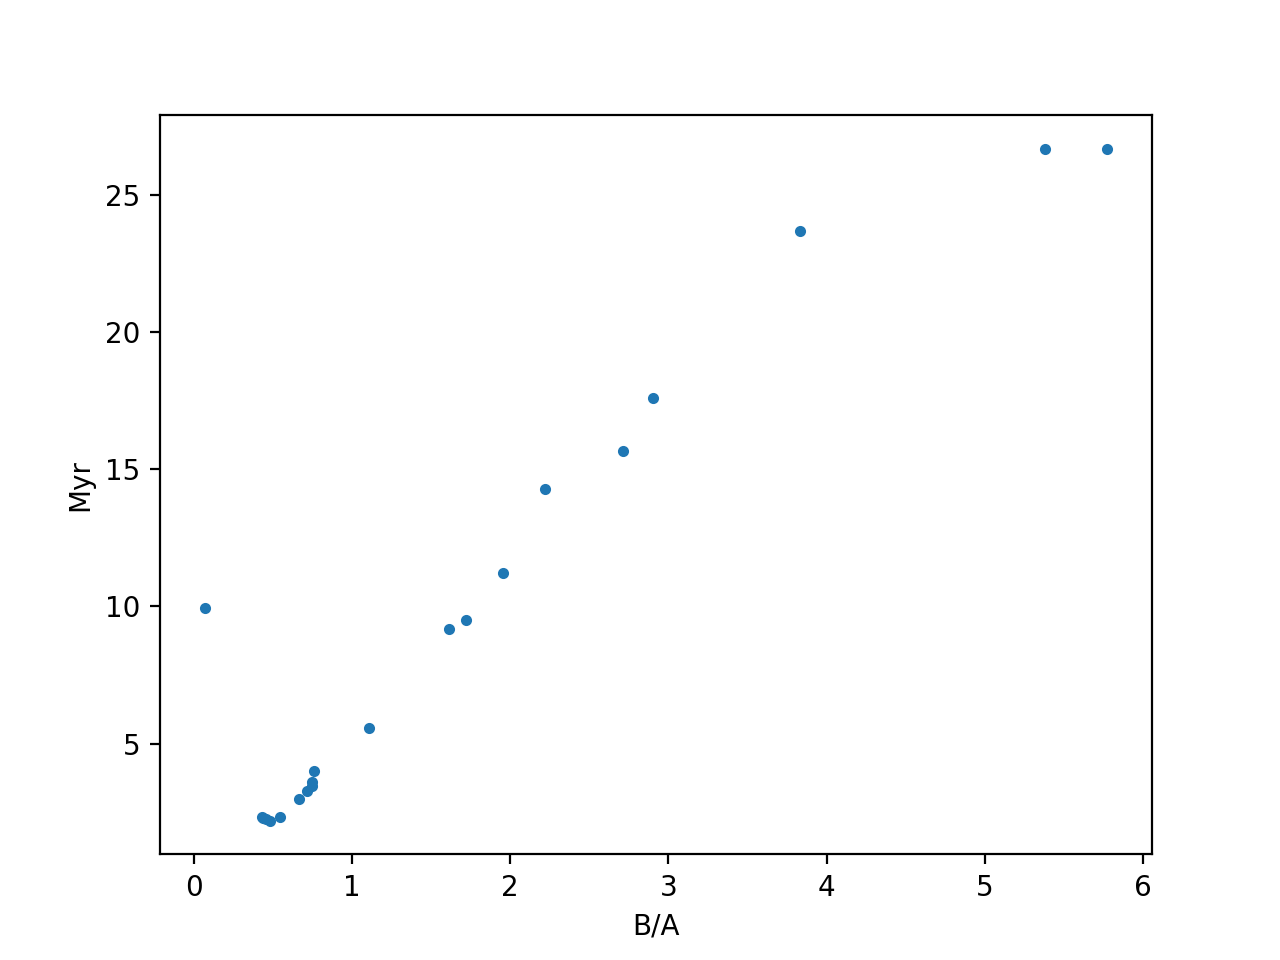
\includegraphics[width=1.\linewidth]{fig2g}
    \caption{Time it takes to reach r=$10^-7$ against B/A}
    \end{figure}
    
    The above figure is constructed by randomly choosing A and B from uniform distribution [0.5,10]. When B/A is smaller then 0.5, the time the black hole needs to reach Schwarzschild radius. B is black hole mass times stellar density, so the smaller it is, the less friction there is acting on the black hole. Then, the black hole will loss energy at a very slow rate, so it takes a long time to reach Schwarzschild radius. When B/A is high, B is high or A is small. In either case, the friction would be huge, which slows the black hole down when it tries to speed up, so it takes a long time to actually reach the Schwarzschild radius. There is clearly a critical case at around B/A=0.5, and that is when the friction is just right, so that the black hole approaches Schwarzschild radius the fastest. A great analogy would be a critically damped oscillator, which reaches equilibrium the fastest, comparing to underdamped or overdamped cases. There also seems to be an asymtop at time=8 Myr.
    
    \item
    First of all, it is clear from the previous section that the actual value of A or B does not matter, only their ratio does. This is true because in the last section, the graph was generated using random number generator. A pair of A and B were chosen from a uniform transformation form 0.5 to 10, and the resulting graph looks like what A or B actually equals to doesn't matter, only their ratio does. Second of all, the initial velocity does not appear to influence how the graph looks either. This is true because I have generated another graph, using a different initial velocity.
    
    \begin{figure}[h]
    \centering
    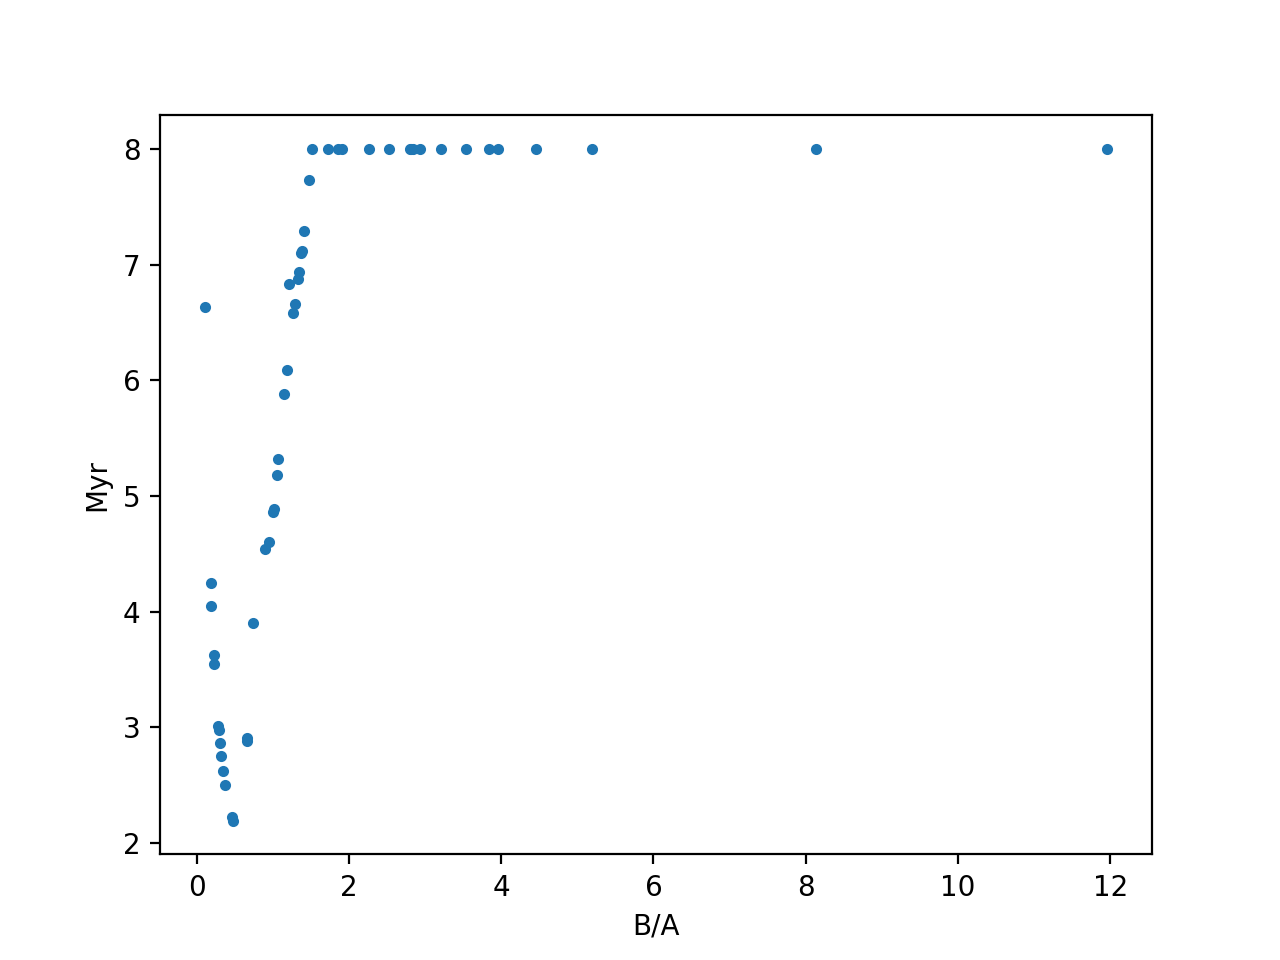
\includegraphics[width=1.\linewidth]{fig2f}
    \caption{Time it takes to reach r=$10^-7$ against B/A, initial velocity =  0.7*$v_{circle}$}
    \end{figure}
    From the above graph, it is clear that slight perturbation would not affect the feature of this plot. (We are not considering the case which we set the initial velocity to infinite so that the two black holes escapes each other, of course)
    
\end{enumerate}

\end{document}
